Dans ce chapitre, l'objectif est de fournir une explication détaillée de l'implémentation de chaque composant du projet, en mettant en évidence les choix techniques qui ont été faits.
Cela permet de donner une vue d'ensemble du projet et d'expliquer les raisons pour lesquelles chaque partie a été mise en place de cette manière spécifique.

\section{Matériel}

Pour la mise en place et les tests de ce projet, plusieurs composants matériels sont nécessaires.

Tout d'abord, il est nécessaire d'avoir une unité qui agit comme le maître I2C.
Dans ce cas, un Raspberry Pi modèle 3 a été utilisé.
Il est possible d'utiliser une autre carte, à condition qu'elle permette d'installer un système d'exploitation capable d'exécuter du code Python.
De plus, il est important d'avoir une connexion I2C disponible.
Dans ce projet, le Raspberry Pi est équipé de Raspbian.

Ensuite, des cartes de développement sont nécessaires pour tester rapidement le code.
STMicroelectronics fournit une gamme de cartes Nucleo équipées de microcontrôleurs STM32.
La carte NUCLEO-G071RB possède un microcontrôleur STM32 très similaire à celui sélectionné pour ce projet, ce qui la rend idéale pour les tests.
De plus, elle est équipée d'un connecteur ST-Link qui permet de programmer le microcontrôleur directement depuis un ordinateur via USB.
Étant donné que c'est une carte de développement, il est facile de connecter des éléments au microcontrôleur via les GPIO.

\begin{figure}[H]
    \centering
    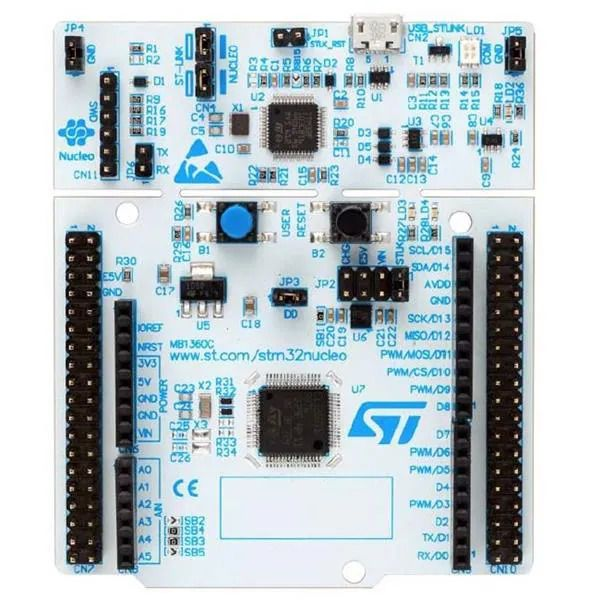
\includegraphics[scale=0.2]{./assets/figures/nucleo.jpg}
    \caption{\cite{nucleo} Carte Nucleo}
\end{figure}

En cas de problème sur le bus I2C, un analyseur logique peut être utile pour observer ce qui se passe.
Dans ce projet, un Saleae Logic 8 a été utilisé.
Cet analyseur logique est pratique pour diagnostiquer les problèmes de communication.
Il permet souvent d'identifier quel composant pose problème et de cibler plus rapidement la source du dysfonctionnement.

En résumé, avec un Raspberry Pi, plusieurs cartes Nucleo servant d'esclaves I2C, il est possible de tester l'intégralité du projet.

\section{Logiciels}

Dans cette section, les différents logiciels utilisés dans ce projet seront décrits, en mettant en évidence leur utilité, leur fonctionnement, ainsi que leurs avantages et inconvénients.

\subsection{PlatformIO}

PlatformIO est un environnement de développement intégré (IDE) qui se présente sous la forme d'une extension pour Visual Studio Code.
Il offre la gestion de plus de cinquante plateformes, plus de vingt \textit{\gls{framework}}s et plus de treize mille bibliothèques.
Cet outil est particulièrement pratique pour explorer rapidement et facilement les différents \textit{\gls{framework}}s compatibles avec les cartes de développement.
Dans le cadre de ce projet, il a été utilisé pour explorer les différentes options de \textit{\gls{framework}}s.
Son principal avantage réside dans sa polyvalence, car il permet de gérer un large éventail de plateformes et de \textit{\gls{framework}}s.
Cependant, sa polyvalence peut également être considérée comme un inconvénient, car il n'est pas optimisé pour un \textit{\gls{framework}} spécifique.

\subsection{Mbed Studio}

Mbed Studio est un environnement de développement intégré (IDE) développé par Arm pour les microcontrôleurs.
Il est basé sur Visual Studio Code et est spécifiquement optimisé pour les microcontrôleurs.
Mbed Studio permet de gérer les cartes de développement de STMicroelectronics, mais il est également possible d'ajouter des cartes de développement d'autres fabricants.
L'un des avantages majeurs de Mbed Studio est sa facilité de débogage, car il permet de déboguer le code directement sur une carte de développement.
Cette fonctionnalité s'avère très pratique lorsqu'on rencontre des comportements indéterminés dans le code.

Dans ce projet, Mbed Studio a été utilisé une fois que le \textit{\gls{framework}} Mbed a été choisi.
Il a permis de gagner du temps en facilitant le processus de débogage.

\section{Mise à jour du micrologiciel}

Dans cette section, le processus de mise à jour du micrologiciel via le bus I2C sera expliqué en détail.
Les deux méthodes possibles pour effectuer la mise à jour seront présentées, en mettant en avant leurs avantages et leurs inconvénients respectifs.

Il existe deux approches pour la mise à jour du micrologiciel via le bus I2C.
La première méthode consiste à télécharger le nouveau micrologiciel à partir de l'application exécutée par le microcontrôleur.
Cela nécessite que le microcontrôleur dispose d'une quantité suffisante de mémoire pour stocker les deux micrologiciels.
Ainsi au redémarrage, le chargeur de démarrage remplace l'ancien micrologiciel par le nouveau.
Cependant, cette méthode nécessite une capacité de mémoire plus importante, car elle nécessite le stockage des deux micrologiciels.

La deuxième méthode consiste à aller dans le chargeur de démarrage pour effectuer la mise à jour.
Dans ce mode, le microcontrôleur est capable de recevoir le nouveau micrologiciel et de le programmer en mémoire.
Cette approche évite le besoin de stocker les deux micrologiciels simultanément, mais elle nécessite que le chargeur de démarrage soit équipé de la fonctionnalité de mise à jour complète.

Chaque méthode présente ses avantages et ses inconvénients.
La première méthode permet une mise à jour plus facile et rapide à partir de l'application, mais elle nécessite une mémoire plus importante.
La deuxième méthode nécessite une fonctionnalité de mise à jour dans le bootloader, mais elle peut être utilisée même si la mémoire disponible est limitée.

\subsection{Envoi du micrologiciel}

L'envoi du micrologiciel se fait par morceaux étant donné que la mémoire vive du microcontrôleur ne peut pas contenir le micrologiciel complet en même temps, en raison de l'utilisation de la mémoire vive par l'application en cours d'exécution.
Les données du micrologiciel sont stockées dans un tampon déclaré dans le code, qui lui est stocké dans la mémoire vive.

La mémoire vive du microcontrôleur choisi a une capacité de 36 kilo-octets.
La taille d'un micrologiciel avec Mbed, incluant une simple réponse I2C, est d'environ 30 kilo-octets.
L'ajout de fonctionnalités supplémentaires augmentera la taille du micrologiciel.

La taille des morceaux a été fixée à 1024 octets. Cette valeur a été sélectionnée pour sa facilité de représentation en termes du nombre de morceaux qui seront envoyés pour le micrologiciel.
De plus, cette taille s'adapte parfaitement à la mémoire vive, même en cas d'utilisation intensive.
Il s'agit d'une taille pertinente qui permet d'optimiser le temps d'envoi en termes du nombre de morceaux, tout en minimisant le temps d'écriture sur la mémoire flash entre deux communications I2C.

\subsection{Detection d'un micrologiciel valide}

Il est impératif que le chargeur de démarrage détecte la présence d'un micrologiciel.
Pour une détection rapide, l'application Mbed comporte une en-tête pré-définie contenant des informations spécifiques.
La première information est un nombre magique, identique à chaque fois et préalablement connu par le chargeur de démarrage.
Ainsi, ce dernier peut simplement vérifier si la première donnée de l'en-tête correspond effectivement au nombre magique prévu.

Ensuite, il est nécessaire de garantir la validité du micrologiciel.
Pour cela, Mbed permet d'ajouter un code de \gls{crc} dans l'en-tête de l'application, qui est automatiquement calculé lors de la génération de l'application.
Le chargeur de démarrage peut alors calculer le \gls{crc} de l'application et le comparer à celui de l'en-tête.
Si les deux \gls{crc} correspondent, cela signifie que le micrologiciel est valide.

Le \gls{crc} est un mécanisme utilisé pour détecter les erreurs de transmission de données.
Il consiste à générer un code de contrôle en effectuant des calculs mathématiques sur les données à transmettre.
Comme il s'agit d'un calcul, il peut être recalculé lors de la réception.

Grâce à ces vérifications, il est assuré que le micrologiciel est valide et que le démarrage de l'application est possible.

\subsection{Mise à jour par l'application}

Dans cette solution, l'utilisateur envoie les données du nouveau micrologiciel directement à l'application s'exécutant sur le microcontrôleur.
L'application reçoit un morceau de données via le bus I2C et l'écrit dans une zone mémoire réservée au nouveau micrologiciel dans la mémoire flash.
Une fois toutes les données du micrologiciel reçues, le microcontrôleur redémarre.
Le chargeur de démarrage doit détecter la présence d'un nouveau micrologiciel dans la zone mémoire réservée.
S'il détecte un micrologiciel valide, il peut le copier à la place de l'ancien micrologiciel.
Une vérification est ensuite effectuée pour s'assurer que la copie s'est déroulée correctement.

Pour implémenter cette solution, lors de la communication I2C entre le maître et le microcontrôleur, un numéro de registre doit être spécifié.
Ce numéro indique à l'application qu'il s'agit d'un message de mise à jour du micrologiciel.
Étant donné que le nouveau micrologiciel est divisé en morceaux, il est nécessaire d'envoyer à la fois le numéro du morceau et le nombre total de morceaux.
Ainsi, l'application peut placer correctement les données dans la mémoire flash.

\begin{figure}[H]
    \centering
    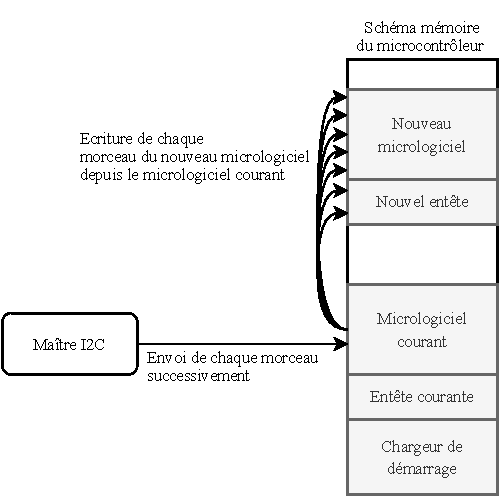
\includegraphics[scale=1.3]{./assets/figures/firmware_update.pdf}
    \caption{Schéma de mise à jour par l'application}
\end{figure}

\subsection{Mise à jour par le chargeur de démarrage}

Dans cette solution, la responsabilité de la mise à jour du micrologiciel repose sur le chargeur de démarrage.
Lorsque l'application du microcontrôleur reçoit l'indication de mettre à jour le micrologiciel via I2C, elle redémarre pour permettre au chargeur de démarrage de prendre le relais.
Cependant, il est nécessaire d'informer le chargeur de démarrage d'attendre une mise à jour et de ne pas démarrer sur le micrologiciel actuel.
Pour ce faire, le chargeur de démarrage s'arrête et attend une mise à jour dans certaines conditions :

\begin{itemize}
    \item L'application doit être mise à jour.
    \item L'application ne présente pas le bon nombre magique.
    \item L'application ne présente pas le bon \gls{crc}.
\end{itemize}

L'application peut se qualifiée de "sujette à mise à jour".
En conséquence, le chargeur de démarrage peut être programmé pour attendre une mise à jour tant que le nombre magique et le \gls{crc} sont corrects.

Une fois que le chargeur de démarrage sait qu'il doit attendre une mise à jour, il reste en attente de la mise à jour via le bus I2C.
Une fois que le nouveau micrologiciel est reçu et vérifié, le chargeur de démarrage démarre avec le nouveau micrologiciel.
Le système de mise à jour a été influencé par la référence \cite{reindl2020software}.

\begin{figure}[H]
    \centering
    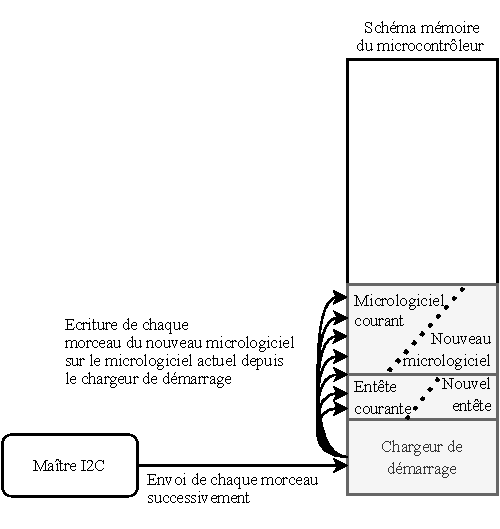
\includegraphics[scale=1.3]{./assets/figures/bootloader_update.pdf}
    \caption{Schéma de mise à jour par le chargeur de démarrage}
\end{figure}

L'avantage de cette solution réside dans la possibilité de mettre à jour le micrologiciel même si l'application est corrompue ou si elle ne gère pas correctement le redémarrage vers le chargeur de démarrage.
Toutefois, la gestion du bus I2C peut être effectuée par le chargeur de démarrage ou par le micrologiciel.

\subsection{Stockage des métadonnées}

Il est nécessaire de permettre la mise à jour du micrologiciel tout en préservant les métadonnées associées.
Cela implique de conserver le nom, le groupe et le type de capteur.
La perte de ces informations à chaque mise à jour serait incohérente.
Par conséquent, il est essentiel de stocker ces données en dehors de la zone mémoire du micrologiciel.
Cependant, elles ne doivent pas faire partie du chargeur de démarrage commun à tous les périphériques.

La solution consiste à réserver une zone mémoire entre le chargeur de démarrage et le micrologiciel.
Ainsi, le micrologiciel peut être mis à jour tout en conservant ses métadonnées, sans les inscrire dans le chargeur de démarrage.

Pour mettre cela en \oe{}uvre, il est nécessaire de réserver plus d'espace pour le chargeur de démarrage.
Cela augmentera sa taille, mais n'utilisera pas la fin de la zone mémoire réservée. Pour faciliter l'effacement et l'écriture des données, il est préférable de choisir une taille de données correspondant à celle d'un secteur pour le microcontrôleur.
Cela permettra aux fonctions d'écriture et d'effacement de mbed de fonctionner de manière optimale.
En effet, la gestion de la mémoire flash se fait par secteurs.
Par conséquent, il est préférable d'adapter la taille réservée pour les métadonnées à la taille d'un secteur et de l'aligner correctement.

Grâce à cette méthode, il est possible de stocker des données liées à une carte qui peuvent être modifiées à la fois par le chargeur de démarrage et par le micrologiciel, tout en maintenant leur intégrité même après une mise à jour complète du micrologiciel.

\begin{figure}[H]
    \centering
    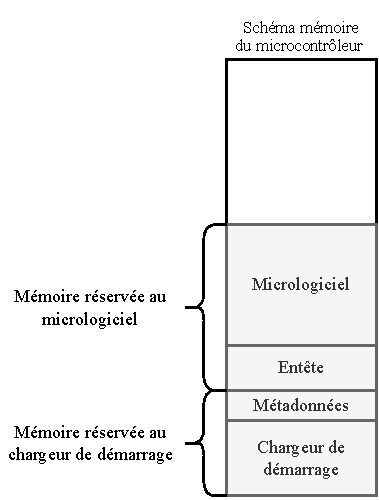
\includegraphics[scale=1.3]{./assets/figures/metadata.pdf}
    \caption{Schéma de la répartition mémoire du microcontrôleur avec les métadonnées}
\end{figure}

\section{Interface POSIX}

Dans cette section, la mise en \oe{}uvre de l'interface POSIX sera détaillée. L'explication des raisons pour lesquelles l'interface a été mise en \oe{}uvre de cette manière et les choix effectués seront abordés.

\subsection{Environnement}

Dans ce projet, aucun environnement matériel final n'est défini. L'objectif consiste à créer un écosystème sur le bus I2C qui peut être réutilisé par d'autres projets. Par conséquent, une interface doit être développée pour être utilisée avec la plupart des maîtres I2C.

Il existe deux types de maîtres I2C possibles. Un maître équipé d'un système d'exploitation, généralement Linux, et un maître sans système d'exploitation, généralement un microcontrôleur. Il convient toutefois de noter qu'une fonctionnalité importante de l'interface POSIX est le déploiement de nouveaux micrologiciels. Par conséquent, le maître I2C doit être capable de mettre à jour, puis de compiler et finalement d'envoyer le micrologiciel.

\subsection{Choix du langage}

En prenant en compte les deux types de maîtres possibles, il convient de déterminer lequel est plus approprié à mettre en avant.
Étant donné la nécessité de modifier et de compiler le code avant de pouvoir l'envoyer, il est peu pertinent de privilégier le maître basé sur un microcontrôleur avec l'écosystème développé.
Par conséquent, il est plus intéressant de construire une interface fonctionnant sur un système d'exploitation. Les explications d'implémentation détaillées permettront, si nécessaire, de créer une interface adaptée à un environnement plus spécifique.

Plusieurs options sont envisageables en ce qui concerne le langage de programmation.
Il est possible d'opter pour un langage tel que C ou C++, ou bien de se tourner vers Python.
Étant donné qu'il s'agit davantage de scripts avancés que d'un véritable programme, il est plus intéressant d'utiliser Python.
Il convient parfaitement à la réalisation d'une interface POSIX et bénéficie de bibliothèques facilitant le développement.

\subsection{Fonctionnement}

Dans cette sous-section, l'objectif consiste à expliquer l'implémentation de chaque partie de l'interface POSIX.
Cela permet de comprendre les choix effectués et d'adapter l'interface POSIX en fonction des besoins spécifiques.

\subsubsection{Mise à jour du micrologiciel}

\todo{Fonctionnement de la mise à jour du micrologiciel}

\subsubsection{Analyse du bus}

\todo{Fonctionnement de l'analyse du bus}

\section{Gestion des erreurs}

\todo{Expliquer le watchdog qui au bout de 5 secondes redémarre la carte}